\documentclass[12pt]{article}
\usepackage{amsmath}
\usepackage{amssymb}
\usepackage{listings}
\usepackage{framed}
\usepackage{graphicx}
\usepackage{algorithm}
\usepackage{algorithmicx}
\usepackage{algpseudocode}

\author{Sean White, Kierstyn Brandt, Rostik Mertz, Norman Tang}
\title{CSCI 432 - Assignment G3}

\begin{document}
\maketitle

\noindent
\textbf{Question A:} For this question, consider the handout and/or CLRS 7.4, which analyze Randomized Quicksort. Consider now the psuedocode we developed in class (where we randomized the order of the array, then ran ‘vanilla’ Quicksort). In your own words, analyze the runtime of our version of Randomzied Quicksort.\\

The difference between 'vanilla' quicksort and our randomized quicksort is we shuffle the array at each iteration and always pick the first element as our pivot. On average we will be splitting the array in two at each iteration, then randomizing in linear time. This gives us $T(n) = 2T(\frac{n}{2}) + \Theta(n)$. Master's theorem is described as $aT(\frac{n}{b}) +f(n)$, in this case both a and b are 2, so $T(n) = \Theta(n^{log_2 (2)log(n)} = \Theta(n log(n))$.\\ 

\noindent
\textbf{Question B:} Algorithms where we use randomization to find a deterministic answer are known as Las Vegas algorithms. Monte Carlo algorithms also use randomization, but might not always give the right answer; however, they either have a high probability of being correct or close to correct.\\

\noindent
(a) Give a Monte Carlo algorithm to estimate $\pi$\\

Given a circle within a square with a side length of A, randomly place n amounts of points in the square, then count the number of points that land within the circle $n_c$, multiply by 4, and divide by the total number of points: 

\begin{align*}
\pi = \frac{4n_c}{n}
\end{align*} \\

\noindent
(b) Let n be the number of random numbers used by your algorithm. Explain why as $n \rightarrow \infty$, the expectation of the output for your algorithm is $\pi$.\\

As n approaches infinity we converge on the true value of $\pi$ because with more points we get a more acurate answer, so if we use all the points we will end up with the true value.\\

\noindent
(c) Implement this algorithm and plot a line graph of the values returned for at least 10 values of n.

\begin{verbatim}
import matplotlib.pyplot as plt
import random
import math

def monteCarloPi(a, n):
    """
    Calculates the value of pi and creates a graph

    Input
    -------
    a - length of the side of the square
    n - number of points
    """
    r = 0.5 * a
    n_c = 0

    for i in range(n):
        x = random.uniform(0, a)
        y = random.uniform(0, a)

        if(math.sqrt((x - r)**2 + (y - r)**2) <= r): # Pythagorean identity
            n_c += 1

    return (4 * n_c)/n

vals = []

for i in range(1,10):
    val = monteCarloPi(1000,i*100)
    vals.append(val)

plt.plot(range(1,10),vals)
plt.show()
\end{verbatim}

The code above generate the following graph:

\begin{figure}[H]
\centerline{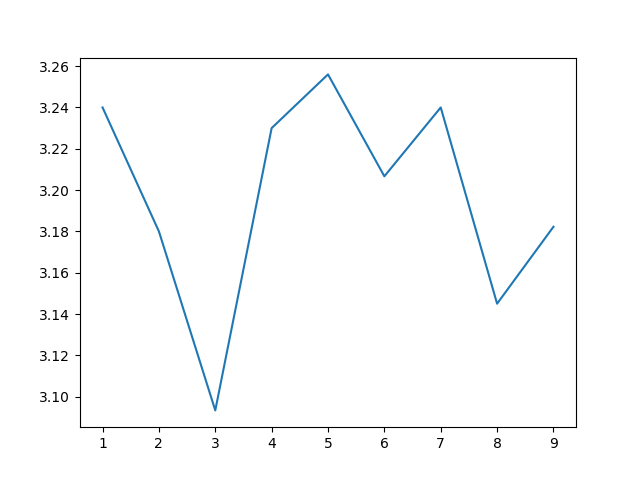
\includegraphics{Figure_1}}
\end{figure}

This is what it lloks like for 100 values of n:

\begin{figure}[H]
\centerline{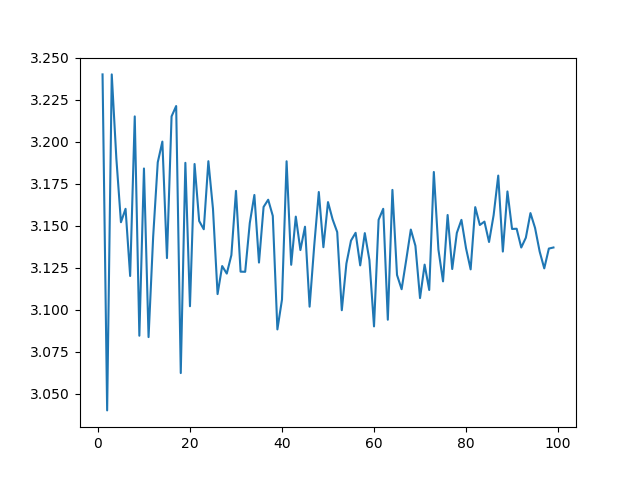
\includegraphics{Figure_2}}
\end{figure}

\end{document}